%% LyX 2.3.6.1 created this file.  For more info, see http://www.lyx.org/.
%% Do not edit unless you really know what you are doing.
\documentclass[english]{article}
\usepackage[T1]{fontenc}
\usepackage[latin9]{inputenc}
\usepackage{geometry}
\geometry{verbose,tmargin=2.5cm,bmargin=2.5cm,lmargin=2.5cm,rmargin=2.5cm}
\usepackage{textcomp}
\usepackage{graphicx}
\PassOptionsToPackage{normalem}{ulem}
\usepackage{ulem}

\makeatletter

%%%%%%%%%%%%%%%%%%%%%%%%%%%%%% LyX specific LaTeX commands.
%% Because html converters don't know tabularnewline
\providecommand{\tabularnewline}{\\}

\makeatother

\usepackage{babel}
\begin{document}
{[}SPLIT\_HERE{]}
\begin{enumerate}
\item \textbf{{[}IJC/PRELIM/9597/2018/P1/Q1{]} }

Customers of coffee shops in Singapore use \textquoteleft codewords\textquoteright{}
to order their drinks. \texttt{DRINKS.TXT} is a text file containing
the codewords. Brewed coffee drinks begin with the word \textquoteleft Kopi\textquoteright ,
while brewed tea drinks begin with the word \textquoteleft Teh\textquoteright .
All other drinks are classified as \textquoteleft Other drinks\textquoteright .

The task is to read the codewords from the file and display a list
according one of the following search criterion:
\begin{enumerate}
\item[1.]  Brewed coffee 
\item[2.]  Brewed tea
\item[3.]  Other drinks
\end{enumerate}

\subsection*{Task 1.1 }

Design and write program code to:
\begin{itemize}
\item read the entire contents of \texttt{DRINKS.TXT} to an appropriate
data structure called \texttt{Drinklist} 
\item display a menu with the following options: 
\noindent \begin{center}
\begin{tabular}{|l|}
\hline 
Menu\tabularnewline
1. Brewed coffee\tabularnewline
2. Brewed tea\tabularnewline
3. Other drinks\tabularnewline
\hline 
\end{tabular}
\par\end{center}
\item \textbullet{} generate the list of drinks and the total number of
items according the user\textquoteright s selection.
\end{itemize}
Example run of the program: 

\textbf{DrinkList} 

Kopi 

Kopi Siew Dai 

Teh O 

Milo Dinosaur 

Clementi 

The output generated from the selection of option 1 would be: 

\textbf{Brewed coffee}

Kopi 

Kopi Siew Dai 

Total items: 2 

\subsection*{Evidence 1 }

Your program code. Screenshot of the output for the selection of Menu
Option 3. \hfill{}{[}15{]}

{[}SPLIT\_HERE{]}
\item \textbf{{[}IJC/PRELIM/9597/2018/P1/Q2{]} }

In a school, students are identified by student numbers. These numbers
are stored in a hash table which uses the hashing function 
\noindent \begin{center}
\texttt{Address <- StudentNumber MOD X }
\par\end{center}

The hash table is implemented as a one-dimensional array with elements
indexed \texttt{0} to\texttt{ (X-1)}. 

\subsection*{Task 2.1}

Write program code to: 
\begin{itemize}
\item Read student numbers from a text file and store them in a hash table.
For the purpose of testing the program, \texttt{X} is to be set to
the value of 12. 

Assume different student numbers will hash to different addresses
(no collisions).
\item Print out the contents of the hash table in the order in which the
elements are stored in the array.
\end{itemize}
Use \texttt{KEYS.TXT} to test your program code.

\subsection*{Evidence 2}

Your program code. 

Screenshot of the program output. \hfill{}{[}7{]}

\subsection*{Task 2.2 }

Linear probing is a method to handle collisions. This means that a
collision is resolved by searching sequentially from the hashed address
for an empty location and storing the student number at this empty
location. If the end of the table is reached, the search for an empty
location is continued from the start of the table.

Use \texttt{KEYS2.TXT} to test your amended program code.

\subsection*{Evidence 3}

Your amended program code which performs linear probing. 

Screenshot of the program output. \hfill{}{[}4{]}

\subsection*{Task 2.3 }

Add code to your Task 2.2 program. The program is to: 
\begin{itemize}
\item Take as input a student number 
\item Search the hash table and output the address (index number) of the
hash table where the student number was found.
\end{itemize}
Use KEYS2.TXT to test your program code. Run the program three times.
Use the following inputs: 15, 23, 88. 

\subsection*{Evidence 4}

Your program code.

Screenshot of the program output.\hfill{} {[}7{]}

{[}SPLIT\_HERE{]}
\item \textbf{{[}IJC/PRELIM/9597/2018/P1/Q3{]} }

A binary tree structure is used to store the names of animals in the
Singapore Zoo. Each animal\textquoteright s name is unique. The binary
tree abstract data type (ADT) has commands to create a new tree, add
data items and print the tree.

The sequence of commands:

\noindent %
\noindent\begin{minipage}[t]{1\columnwidth}%
\texttt{CreateTree() }

\texttt{AddToTree('Tiger') }

\texttt{AddToTree('Lemur') }

\texttt{AddToTree('Bat') }

\texttt{AddToTree('Yak') }

\texttt{AddToTree('Ostrich') }

\texttt{AddToTree('Raccoon') }

\texttt{AddToTree('Macaw')}

\texttt{AddToTree('Zebra')}%
\end{minipage}

would create the following binary tree:
\begin{center}
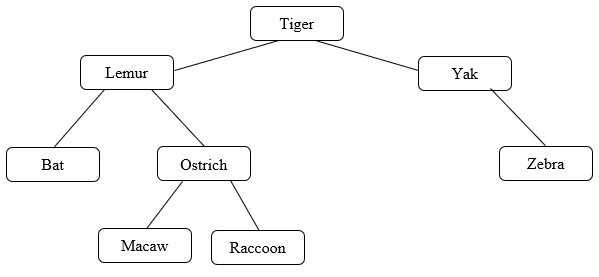
\includegraphics[width=0.5\paperwidth]{C:/Users/Admin/Desktop/Github/question_bank/LyX/static/img/9597-IJC-2018-P1-Q3}
\par\end{center}

The program to implement the ADT will use the classes Tree and Node
designed as follows:
\begin{center}
\begin{tabular}{|l|}
\hline 
\texttt{\hspace{0.25\columnwidth}Tree}\tabularnewline
\hline 
\texttt{thisTree : ARRAY of Node}\tabularnewline
\texttt{root : INTEGER}\tabularnewline
\hline 
\texttt{constructor()}\tabularnewline
\texttt{add(newItem)}\tabularnewline
\texttt{print()}\tabularnewline
\tabularnewline
\tabularnewline
\tabularnewline
\hline 
\end{tabular}%
\begin{tabular}{|l|}
\hline 
\texttt{\hspace{0.25\columnwidth}Node}\tabularnewline
\hline 
\texttt{data : STRING}\tabularnewline
\texttt{leftPtr : INTEGER}\tabularnewline
\texttt{rightPtr : INTEGER }\tabularnewline
\hline 
\texttt{constructor()}\tabularnewline
\texttt{setData(s : STRING)}\tabularnewline
\texttt{setLeftPtr(x : INTEGER)}\tabularnewline
\texttt{setLeftPtr(x : INTEGER)}\tabularnewline
\texttt{getData() : STRING}\tabularnewline
\texttt{getLeftPtr() : INTEGER }\tabularnewline
\texttt{getRightPtr() : INTEGER}\tabularnewline
\hline 
\end{tabular}
\par\end{center}

The program code will do the following:
\begin{itemize}
\item Create a new tree, which has: 
\begin{itemize}
\item no nodes 
\item the root set to --1 
\end{itemize}
\item Use the root as a pointer to the first node in the tree
\item Add a new node to the tree in the appropriate position. The left and
right pointers of this node should have the initial value of --1. 
\item Use the \texttt{print()} method to output, for each node, in array
order: 
\begin{itemize}
\item the data item
\item the left pointer 
\item the right pointer.
\end{itemize}
\end{itemize}

\subsection*{Task 3.1 }

Write program code to define the classes \texttt{Tree} and \texttt{Node}.

\subsection*{Evidence 5}

Your program code. \hfill{}{[}26{]}

\subsection*{Task 3.2}

The program is to be tested. Write a sequence of program statements
to:
\begin{itemize}
\item create a new tree 
\item add the data items as shown in the sequence of commands on the previous
page 
\item print the array contents.
\end{itemize}
Execute your program to test it.

\subsection*{Evidence 6 }

Your program code.

Screenshot of test run. \hfill{}{[}3{]}

\subsection*{Task 3.3 }

A method \texttt{postOrderTraversal()} is to be added. This left-to-right
post-order traversal outputs the data stored in the child nodes before
outputting the data stored in the root node. 

Write program code to:
\begin{itemize}
\item implement this method
\item Test the program code with the data from Task 3.2.
\end{itemize}

\subsection*{Evidence 7 }

Your program code. 

Screenshot of test run.\hfill{} {[}7{]}

{[}SPLIT\_HERE{]}
\item \textbf{{[}IJC/PRELIM/9597/2018/P1/Q4{]} }

Bowling is a sport in which a \textquoteleft bowler\textquoteright{}
rolls a bowling ball down a synthetic lane and towards ten pins positioned
at the end of the lane. The objective is to score points by knocking
down as many pins as possible. 
\begin{center}
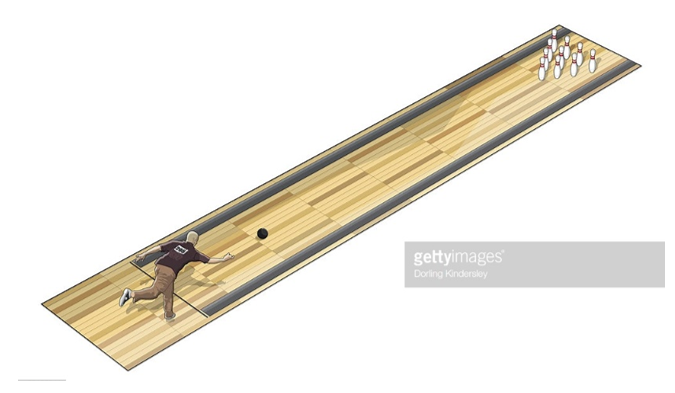
\includegraphics[width=0.5\paperwidth]{C:/Users/Admin/Desktop/Github/question_bank/LyX/static/img/9597-IJC-2018-P1-Q4}
\par\end{center}

\textbf{A bowling game }

One game of bowling consists of ten frames. Each frame consists of
two chances for the bowler to knock down ten pins.

\textbf{Strikes and spares }

Knocking down all ten pins on the first roll of any frame is called
a \textbf{strike}, denoted by \textquoteleft X\textquoteright{} on
the score sheet. If a bowler takes two rolls to knock down all ten
pins, it is called a \textbf{spare}.

\textbf{Scoring and bonus scoring}

Each pin that is knocked down is worth 1 point. 

A strike is worth 10 points plus the number of pins hit on the next
two rolls.

A spare is worth 10 points plus the number of pins hit on the next
roll.

The total score for a game ranges from 0 to 300 points.

\textbf{The tenth frame }

A bowler who strikes or spares the tenth frame will be given one extra
roll. The number of pins hit on this roll will be added to the bowler\textquoteright s
score.

\textbf{Sample Scores} 

\begin{tabular}{|c|c|c|c|c|c|c|c|c|c|c|}
\hline 
Frame & 1 & 2 & 3 & 4 & 5 & 6 & 7 & 8 & 9 & 10\tabularnewline
\hline 
Result & \textbf{\uline{X}} & 7|\textbf{\uline{3}} & 7|2 & 9|\textbf{\uline{1}} & \textbf{\uline{X}} & \textbf{\uline{X}} & \textbf{\uline{X}} & 2|3 & 6|\textbf{\uline{4}} & 7|\textbf{\uline{3}}|3\tabularnewline
\hline 
Frame Score & 20 & 17 & 9 & 20 & 30 & 22 & 15 & 5 & 17 & 13\tabularnewline
\hline 
Cumulative Score & 20 & 37 & 46 & 66 & 96 & 118 & 133 & 138 & 155 & 168\tabularnewline
\hline 
\end{tabular}

\begin{tabular}{|c|c|c|c|c|c|c|c|c|c|c|}
\hline 
Frame & 1 & 2 & 3 & 4 & 5 & 6 & 7 & 8 & 9 & 10\tabularnewline
\hline 
Result & 0|5 & 8|0 & \textbf{\uline{X}} & 0|5 & \textbf{\uline{X}} & 6|\textbf{\uline{4}} & 0|5 & 8|1 & 9|\textbf{\uline{1}} & 5|0\tabularnewline
\hline 
Frame Score & 5 & 8 & 15 & 5 & 20 & 10 & 5 & 9 & 15 & 5\tabularnewline
\hline 
Cumulative Score & 5 & 13 & 28 & 33 & 53 & 63 & 68 & 77 & 92 & 97\tabularnewline
\hline 
\end{tabular}

\begin{tabular}{|c|c|c|c|c|c|c|c|c|c|c|}
\hline 
Frame & 1 & 2 & 3 & 4 & 5 & 6 & 7 & 8 & 9 & 10\tabularnewline
\hline 
Result & \textbf{\uline{X}} & \textbf{\uline{X}} & \textbf{\uline{X}} & \textbf{\uline{X}} & 9|\textbf{\uline{1}} & \textbf{\uline{X}} & 0|0 & 2|2 & 8|\textbf{\uline{2}} & \textbf{\uline{X}}|X|X\tabularnewline
\hline 
Frame Score & 30 & 30 & 29 & 20 & 20 & 10 & 0 & 4 & 20 & 30\tabularnewline
\hline 
Cumulative Score & 30 & 60 & 89 & 109 & 129 & 139 & 139 & 143 & 163 & 193\tabularnewline
\hline 
\end{tabular}

The following algorithms calculate the total score for a bowling game.

\noindent %
\noindent\begin{minipage}[t]{1\columnwidth}%
\texttt{//Used interchangeably in the code for readability}

\texttt{Ten <- 'X'}

\texttt{Strike <- Ten}

\texttt{\bigskip{}
}

\texttt{//Converting the 'X' or 'number' to INTEGER }

\texttt{FUNCTION Pins(Throw as STRING)}

\texttt{\qquad{}IF Throw = Ten THEN}

\texttt{\qquad{}\qquad{}RETURN 10}

\texttt{\qquad{}ELSE}

\texttt{\qquad{}\qquad{}RETURN INTEGER(Throw)}

\texttt{\qquad{}ENDIF }

\texttt{END FUNCTION}

\texttt{\bigskip{}
}

\texttt{//Recursive Procedure }

\texttt{FUNCTION Bowling\_Score(Throws as STRING)}

\texttt{\bigskip{}
}

\texttt{\qquad{}//Helper function to keep track of current frame
number}

\texttt{\qquad{}FUNCTION Bowling\_Score\_Helper(Throws as STRING,
Frame\_Num as INTEGER) }

\texttt{\bigskip{}
}

\texttt{\qquad{}\qquad{}//Frame 10 with no bonus }

\texttt{\qquad{}\qquad{}IF Frame\_Num = 10 AND LENGTH(Throws) =
2 THEN }

\texttt{\qquad{}\qquad{}\qquad{}RETURN SUM(Pins(Throws{[}0{]}),
Pins(Throws{[}1{]})) }

\texttt{\qquad{}\qquad{}ENDIF}

\texttt{\bigskip{}
}

\texttt{\qquad{}\qquad{}//Frame 10 with bonus}

\texttt{\qquad{}\qquad{}IF Frame\_Num = 10 AND LENGTH(Throws) =
3 THEN}

\texttt{\qquad{}\qquad{}\qquad{}RETURN SUM(Pins(Throws{[}0{]}),Pins(Throws{[}1{]}),Pins(Throws{[}2{]})) }

\texttt{\qquad{}\qquad{}ENDIF}

\texttt{\bigskip{}
}

\texttt{\qquad{}\qquad{}//A Strike }

\texttt{\qquad{}\qquad{}IF Throws{[}0{]} = Strike THEN}

\texttt{\qquad{}\qquad{}\qquad{}Frame\_Score <- 10 + SUM(Pins(Throws{[}1{]}),
Pins(Throws{[}2{]}))}

\texttt{\qquad{}\qquad{}\qquad{}RETURN Frame\_Score + Bowling\_Score\_Helper(Throws{[}1:{]},
Frame\_Num + 1) }

\texttt{\qquad{}\qquad{}ENDIF}

\texttt{\bigskip{}
}

\texttt{\qquad{}\qquad{}Frame\_Score <- SUM(Pins(Throws{[}0{]}),
Pins(Throws{[}1{]}))}

\texttt{\bigskip{}
}

\texttt{\qquad{}\qquad{}//A Spare}

\texttt{\qquad{}\qquad{}IF Frame\_Score = 10 THEN}

\texttt{\qquad{}\qquad{}\qquad{}RETURN 10 + Pins(Throws{[}2{]})
+ Bowling\_Score\_Helper(Throws{[}2:{]}, Frame\_Num + 1)}

\texttt{\qquad{}\qquad{}ENDIF}

\texttt{\bigskip{}
}

\texttt{\qquad{}\qquad{}//Frame with no bonus }

\texttt{\qquad{}\qquad{}RETURN Frame\_Score + Bowling\_Score\_Helper(Throws{[}2:{]},
Frame\_Num + 1)}

\texttt{\qquad{}END FUNCTION}

\texttt{\bigskip{}
}

\texttt{\qquad{}RETURN Bowling\_Score\_Helper(Throws, 1) }

\texttt{END FUNCTION }%
\end{minipage}

Note: The above pseudocode is available in the text file \texttt{PSEUDOCODE\_TASK\_4\_1.TX}T
but with \textquoteleft \texttt{=}\textquoteright{} used in place
of \textquoteleft <-\textquoteright{} shown above.

\subsection*{Task 4.1 }

Write a program to calculate a bowling score using the algorithms
provided on the previous page.

\subsection*{Evidence 8 }

Your program code for Task 4.1.\hfill{} {[}5{]}

\subsection*{Evidence 9 }

Screenshot of the results of the following function calls: 
\begin{enumerate}
\item[1.] \texttt{ Bowling\_Score('X2815X91X365452X0X')}\hfill{} {[}1{]}
\item[2.]  \texttt{Bowling\_Score('91739182X90X90X82X')} \hfill{} {[}1{]}
\end{enumerate}

\subsection*{Task 4.2 }

Draw up a list of \texttt{three} suitable test cases. Complete a table
with the following headings: 
\noindent \begin{center}
\begin{tabular}{|c|c|c|}
\hline 
Bowling Score & Purpose of the test & Expected Output \tabularnewline
\hline 
 &  & \tabularnewline
\hline 
 &  & \tabularnewline
\hline 
 &  & \tabularnewline
\hline 
\end{tabular}
\par\end{center}

Amend your program code to include the handling of the test cases
listed in your table. 

\subsection*{Evidence 10 }

The completed table.\hfill{} {[}3{]}

\subsection*{Evidence 11 }

Your amended program code that includes \textbf{internal commentary}.
\hfill{} {[}3{]}

\subsection*{Evidence 12 }

Screenshots for each test data run. {[}3{]}\quad{} 

At the 2018 Singapore Championship, bowlers play a total of six games
each in the qualifying round. The eight bowlers with the highest total
score qualify for the Masters Competition. You may assume that there
are no bowlers with the same total score.

\texttt{SCORES.TXT} is a text file containing the register number,
country and the scores for six games of twenty bowlers in the qualifying
round, with one bowler per line in the format: 
\noindent \begin{center}
\texttt{<Register Number> <Country> <Score 1> <Score 2> \dots{} <Score
6>}
\par\end{center}

For example: 
\noindent \begin{center}
\texttt{157 MAS XXXXX9091XXX82 90XXXXXXXXXX9 \dots{} 8172XXXX919191XX8}
\par\end{center}

\subsection*{Task 4.3 }

Design and write program code to:
\begin{itemize}
\item Read the entire contents of \texttt{SCORES.TXT}. 
\item Calculate the score of each game for all twenty bowlers, using your
code in \textbf{Evidence 8}. You may assume that all the scores in
\texttt{SCORES.TXT} are valid scores.
\item Calculate the total score for each bowler and store this in an appropriate
data structure together with the respective \texttt{Register Number}
and \texttt{Country}. 
\item Use \textbf{bubble sort} to sort the bowlers according to their total
score. 
\item Output the Official Results of the competition.
\end{itemize}
An example of the output should look like this:
\noindent \begin{center}
\begin{tabular}{cccc}
\multicolumn{4}{c}{\texttt{Official Results}}\tabularnewline
\texttt{Position} & \texttt{Register Number} & \texttt{Country} & \texttt{Total Score}\tabularnewline
\texttt{1} & \texttt{175} & \texttt{SIN} & \texttt{1734}\tabularnewline
\texttt{2} & \texttt{299} & \texttt{SIN} & \texttt{1724}\tabularnewline
\texttt{.} & \texttt{.} & \texttt{.} & \texttt{.}\tabularnewline
\texttt{.} & \texttt{.} & \texttt{.} & \texttt{.}\tabularnewline
\texttt{.} & \texttt{.} & \texttt{.} & \texttt{.}\tabularnewline
\texttt{20} & \texttt{245} & \texttt{MAS} & \texttt{1270}\tabularnewline
\end{tabular}
\par\end{center}

\subsection*{Evidence 13 }

The bubble sort code procedure.\hfill{} {[}4{]}

\subsection*{Evidence 14 }

Your program code for Task 4.3.

Screenshot showing the output.\hfill{} {[}11{]}

{[}SPLIT\_HERE{]}
\item \textbf{{[}IJC/PRELIM/9597/2018/P2/Q1{]} }

The Singapore Armed Forces is made up of many men and women who are
committed to protect the nation\textquoteright s peace and security.
The Ministry of Defence (MINDEF) keeps detailed personnel records
of all servicemen and servicewomen in a large database housed in the
central server at MINDEF Headquarters. Personnel records include career
history, salary, military rank, health details, achievements and awards.

The Human Resource Unit (HR) of MINDEF manages these records regularly
through a computerised system. Updates of the personnel\textquoteright s
records must be done within three working days once HR receives the
information from any military unit in MINDEF. Subsequently, administrative
officers of the military units in MINDEF will be able to view these
records via the intranet.

The current system has been used for the last fifteen years. MINDEF
wishes to replace this system with a new computerised system with
enhanced features and a better user interface. A system developer
is employed to carry out the task. 

MINDEF has accepted the proposal by the system developer, who will
address the following problems with the current system: 

\noindent %
\noindent\begin{minipage}[t]{1\columnwidth}%
\begin{enumerate}
\item[1.]  Poor database design 
\item[2.]  Limited types of reports that can be generated 
\item[3.]  Lack of intuitiveness of the user interface
\item[4.]  Slow system response time 
\item[5.]  Incompatibility with the current devices\textquoteright{} operating
systems
\item[6.]  Minimal security protection
\end{enumerate}
%
\end{minipage}
\begin{enumerate}
\item The system developer produces the following Program Evaluation and
Review Technique (PERT) chart:

A. Analysis of the solution 

B. Design of the solution 

C. Development of the solution

D. Documentation of the solution 

E. Implementation of the solution

F. Testing of the solution

Time is measured in weeks. \quad{} 
\begin{center}
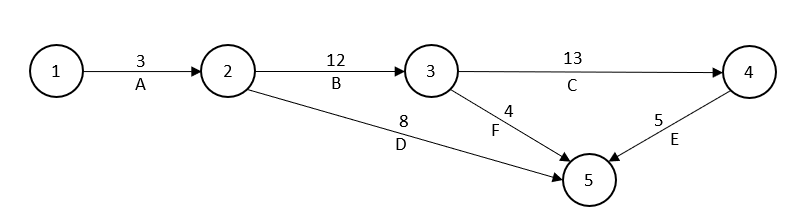
\includegraphics[width=0.5\paperwidth]{C:/Users/Admin/Desktop/Github/question_bank/LyX/static/img/9597-IJC-2018-P2-Q1-1}
\par\end{center}

From the PERT chart, 
\begin{enumerate}
\item state the critical path.\hfill{} {[}1{]}
\item state the minimum time in which the project can be completed. \hfill{}{[}1{]}
\item describe and give an example of concurrent activities. \hfill{}{[}2{]}
\item describe and give an example of dependent activities.\hfill{} {[}2{]}
\end{enumerate}
\item The system developer is required to provide more details in the PERT
chart. It is proposed that Activity F should be removed from the chart
and three new activities added:

J. Black box testing -- 2 weeks 

K. White box testing -- 2 weeks

L. Beta testing -- 3 weeks

Redraw the PERT chart to show the effects of these changes. \hfill{}{[}4{]}
\item Draw a sketch of the Gantt chart to show the information in \textbf{(a)}.
\hfill{}{[}6{]}
\item Maintenance will be required after implementing the new system.

Describe two types of maintenance. For each type, give an example
for this new system. \hfill{}{[}6{]}
\item The new system will provide all staff in HR with full access to all
personnel records. The administrative officers of the military unit
will have only read access to the data. Only designated computers
in the MINDEF network are able to access the system.

Describe \textbf{three} ways in which the security of this system
can be maintained. \hfill{}{[}6{]}
\item MINDEF is considering to allow servicemen and servicewomen to update
their own personnel records directly into the system via the internet.
Describe one security concern and one ethical issue that may arise
due to this proposed implementation.\hfill{} {[}2{]}
\end{enumerate}
{[}SPLIT\_HERE{]}
\item \textbf{{[}IJC/PRELIM/9597/2018/P2/Q2{]} }

A self-checkout counter of a local supermarket, PriceFare, allows
customers to scan and pay for their groceries without the need for
a human cashier. The customer interacts directly via the following
user interface:
\begin{center}
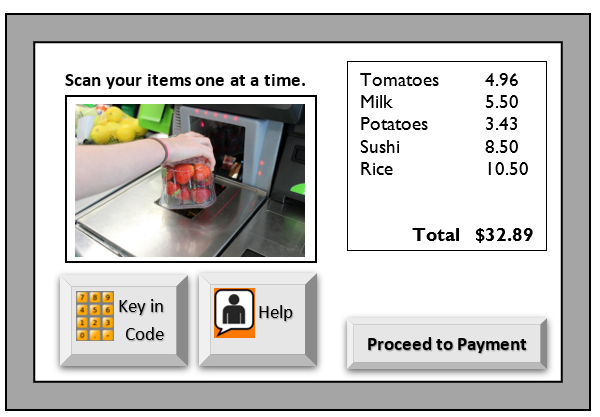
\includegraphics[width=0.5\paperwidth]{C:/Users/Admin/Desktop/Github/question_bank/LyX/static/img/9597-IJC-2018-P2-Q2-1}
\par\end{center}
\begin{enumerate}
\item State the type of user interface being used. \hfill{}{[}1{]}
\item Name \textbf{two} user input methods for the user interface. \hfill{}
{[}2{]}
\item Identify \textbf{one} feature of the user interface and explain the
design consideration involved in the choice of this feature. \hfill{}{[}3{]}
\end{enumerate}
\textquotedblleft Many people confuse the Internet as cloud computing\textquotedblright .
\begin{enumerate}
\item[(d)]  Explain how the Internet and cloud computing are different. \hfill{}{[}2{]}
\end{enumerate}
PriceFare intends to launch an online service in Singapore. Customers
can purchase their groceries using a mobile application anywhere in
Singapore. The management of PriceFare is deciding between two different
types of cloud services for this project -- Platform as a Service
(PaaS) and Infrastructure as a Service (IaaS). 
\begin{enumerate}
\item[(e)]  Describe the differences between PaaS and IaaS. \hfill{} {[}2{]}
\item[(f)]  What should the management of PriceFare consider when choosing between
these two types of cloud services? \hfill{}{[}2{]}
\item[(g)]  Give a reason why Software as a Service (SaaS) is not considered
by the management of PriceFare. \hfill{} {[}1{]}
\end{enumerate}
{[}SPLIT\_HERE{]}
\item \textbf{{[}IJC/PRELIM/9597/2018/P2/Q3{]} }

The following table shows a partial list of Unicode characters. 
\begin{center}
\begin{tabular}{|c|c|c|c|}
\hline 
Unicode & Character & Denary Value & Description\tabularnewline
\hline 
U+0393 & $\Gamma$ & 915 & Greek Capital Letter Gamma\tabularnewline
\hline 
U+0394 & $\Delta$ & 916 & Greek Capital Letter Delta\tabularnewline
\hline 
U+0395 & $E$ & 917 & Greek Capital Letter Epsilon\tabularnewline
\hline 
U+0396 & $Z$ & 918 & Greek Capital Letter Zeta\tabularnewline
\hline 
U+0397 & $H$ & 919 & Greek Capital Letter Eta\tabularnewline
\hline 
U+0398 & $\Theta$ & 920 & Greek Capital Letter Theta\tabularnewline
\hline 
U+0399 & $I$ & 921 & Greek Capital Letter Iota\tabularnewline
\hline 
U+039A & $K$ & 922 & Greek Capital Letter Kappa\tabularnewline
\hline 
\end{tabular}
\par\end{center}
\begin{enumerate}
\item Explain why the Unicode encoding system has replaced ASCII.\hfill{}
{[}2{]}
\item The Greek capital letter Omega, \textquoteleft $\Omega$\textquoteright ,
has denary value 937. Write down its corresponding Unicode.\hfill{}
{[}1{]}
\item Write down the 16-bit binary value of the Unicode character with Unicode
U+0A6C7. \hfill{}{[}1{]}
\end{enumerate}
The following pseudocode for a sort algorithm is used to sort a list
of Greek character names.

\noindent\begin{minipage}[t]{1\columnwidth}%
\texttt{01 FOR i <- 2 TO ArraySize: }

\texttt{02 \qquad{}Key Array{[}i{]} }

\texttt{03 \qquad{}j <- i-1 }

\texttt{04 \qquad{}WHILE (j > 0) and (Key < Array{[}j{]}) }

\texttt{05 \qquad{}\qquad{}Array{[}j+1{]} <- Array{[}j{]}}

\texttt{06 \qquad{}\qquad{}j <- j-1}

\texttt{07 \qquad{}ENDWHILE}

\texttt{08 \qquad{}Array{[}j+1{]} <- Key}

\texttt{09 ENDFOR}%
\end{minipage}

The sort algorithm is used on \texttt{Array}, a list of 5 Greek character
names.
\noindent \begin{center}
\begin{tabular}{c|c|c|c|c|c|}
\cline{2-6} \cline{3-6} \cline{4-6} \cline{5-6} \cline{6-6} 
Array & Gamma & Delta & Epsilon & Zeta & Eta\tabularnewline
\cline{2-6} \cline{3-6} \cline{4-6} \cline{5-6} \cline{6-6} 
\end{tabular}
\par\end{center}
\begin{enumerate}
\item[(d)]  Write down the name of this sort algorithm. \hfill{}{[}1{]}
\item[(e)]  Copy and then complete the trace table given below. \hfill{}{[}6{]}
\noindent \begin{center}
\begin{tabular}{|c|c|c|c|c|c|c|c|}
\hline 
\multicolumn{5}{|c|}{\texttt{Array}} & \multicolumn{3}{c|}{}\tabularnewline
\hline 
\texttt{{[}1{]}} & \texttt{{[}2{]}} & \texttt{{[}3{]}} & \texttt{{[}4{]}} & \texttt{{[}5{]}} & \texttt{i} & \texttt{j} & \texttt{Key}\tabularnewline
\hline 
\texttt{Gamma} & \texttt{Delta} & \texttt{Epsilon} & \texttt{Zeta} & \texttt{Eta} &  &  & \tabularnewline
\hline 
 &  &  &  &  &  &  & \tabularnewline
\hline 
 &  &  &  &  &  &  & \tabularnewline
\hline 
 &  &  &  &  &  &  & \tabularnewline
\hline 
 &  &  &  &  &  &  & \tabularnewline
\end{tabular}
\par\end{center}
\item[(f)]  State the efficiency, in terms of running time, of this sort algorithm
if the Greek character names in Array are initially in reverse order.
\hfill{}{[}1{]}
\end{enumerate}
{[}SPLIT\_HERE{]}
\item \textbf{{[}IJC/PRELIM/9597/2018/P2/Q4{]} }

A large file is to be transmitted between two computers over the internet.
\begin{enumerate}
\item Explain how packet switching is used to transmit the file over the
internet. \hfill{}{[}3{]}
\item The bytes that make up a packet is checked by the receiving computer.
Explain how this can be done for:
\begin{enumerate}
\item[I. ] The individual bytes which make up the packet \hfill{}{[}2{]}
\item[II.]  The collection of bytes which makes up the packet. \hfill{}{[}2{]}
\end{enumerate}
\end{enumerate}
Each packet consists of: 
\begin{itemize}
\item A 3-digit number from 100 to 800 
\item Upper case letters 
\item The <space> character 
\item A start character (\$) and an end character (\$). 
\end{itemize}
An example of a packet is:
\noindent \begin{center}
\texttt{\$TBHIKR 565 KUTGW\$ }
\par\end{center}
\begin{enumerate}
\item[(c)]  Explain the difference between data validation and data verification.
\hfill{}{[}2{]}
\item[(d)]  Describe \textbf{three} validation checks that the receiving computer
should perform on each packet received. \hfill{}{[}6{]}
\end{enumerate}
{[}SPLIT\_HERE{]}\quad{}
\item \textbf{{[}IJC/PRELIM/9597/2018/P2/Q5{]} }

The following security advisory was issued after the recent cyberattack
on SingHealth\textquoteright s IT system.
\begin{center}
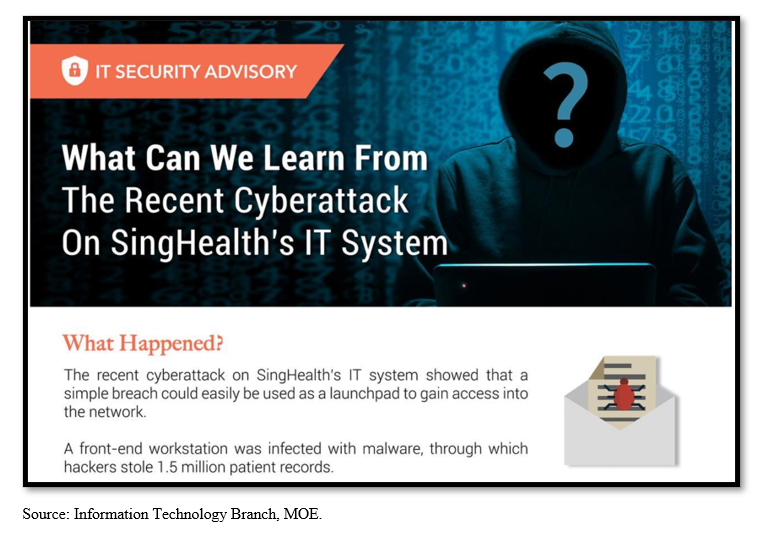
\includegraphics[width=0.5\paperwidth]{C:/Users/Admin/Desktop/Github/question_bank/LyX/static/img/9597-IJC-2018-P2-Q5-1}
\par\end{center}

Employees of SingHealth\textquoteright s group of hospitals are issued
with computing devices, which have access to patients\textquoteright{}
records stored on the SingHealth central server, via the internet.
Each employee is also issued with an email account for both internal
and external communications. 
\begin{enumerate}
\item Describe \textbf{two} differences between a client-server network
and a peer-to-peer network. \hfill{}{[}4{]}

\emph{\textquotedblleft \dots{} a simple breach could easily be used
as a launchpad to gain access into the network.\textquotedblright{}}
\item Describe how a breach could have happened and how patient records
were subsequently accessed. \hfill{}{[}4{]}
\begin{enumerate}
\item A further notice adds that \textquotedblleft \emph{Employees can practice
good personal data protection and cybersecurity habits in their place
of work.}\textquotedblright{}
\end{enumerate}
\item Describe \textbf{two} ways that this can be done. \hfill{} {[}2{]}
\item List \textbf{two} ways that SingHealth as an organisation can do to
ensure the security of their network. \hfill{}{[}2{]}
\end{enumerate}
{[}SPLIT\_HERE{]}
\item \textbf{{[}IJC/PRELIM/9597/2018/P2/Q6{]} }

The Singapore Bowling Federation (SBF) is made up of several affiliate
clubs. To participate in a competition, a competitive bowler is required
to be enrolled in exactly one affiliate club. A relational database
is used by SBF to store data about competition entries and results.
Four tables present in the database are \texttt{CLUB}, \texttt{MEMBER},
\texttt{COMPETITION} and \texttt{COMPETITION-MEMBER}. A new row is
created in the \texttt{COMPETITION-MEMBER} table whenever a competitive
bowler registers for a competition. When the competition results become
available, they are added to the appropriate row.

Each competitive bowler, affiliate club and competition has a unique
identification number.
\begin{enumerate}
\item Explain what a relational database is.\hfill{} {[}2{]}
\item Draw the Entity-Relationship (E-R) diagram to show the relationship
between the four tables that provide for a fully normalised database
design. \hfill{}{[}4{]}
\item A table description can be expressed as:

\texttt{Tablename (}\texttt{\uline{Attribute1}}\texttt{, Attribute2,
Attribute3, \dots ) }

The primary key is indicated by underlining one or more attributes.

Write the table descriptions for the four tables. You should include
at least \textbf{one} other attribute in addition to the primary key.
\hfill{}{[}8{]}
\end{enumerate}
(d) Give \textbf{two} examples of data anomaly and describe how they
may occur if the database that was designed for SBF was not fully
normalised.\hfill{} {[}4{]}

{[}SPLIT\_HERE{]}
\end{enumerate}

\end{document}
